% \documentclass{fp-slides}
\documentclass[10pt,portrait]{beamer}
\usepackage{mathtext}
\usetheme{Warsaw}
\newcommand{\maybepause}{}
%\newcommand{\maybepause}{\pause}
\setlength{\floatsep}{8pt plus 2pt minus 2pt}
\setlength{\textfloatsep}{8pt plus 2pt minus 2pt}
\setlength{\intextsep}{12pt plus 2pt minus 2pt}
\AtBeginDocument{%
% \selectlanguage{russian}%
\frenchspacing
\righthyphenmin=2
\sloppy
%\author{Shiray Andrey}
\institute{O.O.Bogomolets National Medical University}
\title{Biostatistics}
% Basics of statistical processing of biomedical  data
}
\newtheorem{defin}{Definition}[section]
% \ifx\pdfoutput\undefined
% % we are running LaTeX, not pdflatex
% \usepackage{graphicx}
% \else
% % we are running pdflatex, so convert .eps files to .pdf
% \usepackage[pdftex]{graphicx}
% \usepackage{epstopdf}
% \fi 

\usepackage{graphics}
\begin{document}

%%%%%%%%%%%%%%% Define code blocks

% \defverbatim[colored]\factCcode{%
% \begin{lstlisting}[frame=single,language=C]
%   int fact(int n)
%   { int x = 1;
%     while (n > 0)
%      { x = x * n;
%        n = n - 1;
%      }
%     return x;
%   }
% \end{lstlisting}}
% 
% \defverbatim[colored]\factMLcode{%
% \begin{lstlisting}[frame=single]
%   let rec fact n =
%     if n = 0 then 1
%     else n * fact(n - 1);;
% \end{lstlisting}}
% 
% \defverbatim[colored]\badFuncCode{%
% \begin{lstlisting}[frame=single]
%   int rand(void)
%   { static int n = 0;
%     return n = 2147001325 * n + 715136305;
%   }
% \end{lstlisting}}

%%%%%%%%%%%%%%%%%%%%%%

\frame{\titlepage}

% \section*{Biostatistics}

%\subsection{Обсуждаемые темы}


\frame{
  \frametitle{Contents}
 \begin{itemize}
\item Confidence intervals 
\item Evidence-based medicine
\item Clinical trials
\item Hypothesis testing
 \end{itemize}

}

\frame{
  \frametitle{Confidence intervals}
\begin{defin}
\[
  \Pr_{\theta}(u(X)<\theta<v(X))=\gamma\; \forall \theta.
\]
 \begin{itemize}
  \item $\theta$ -- statistical parameter, which is a quantity to be estimated
\item $\gamma$ -- confidence level
 \end{itemize}
\end{defin}
\begin{center}
 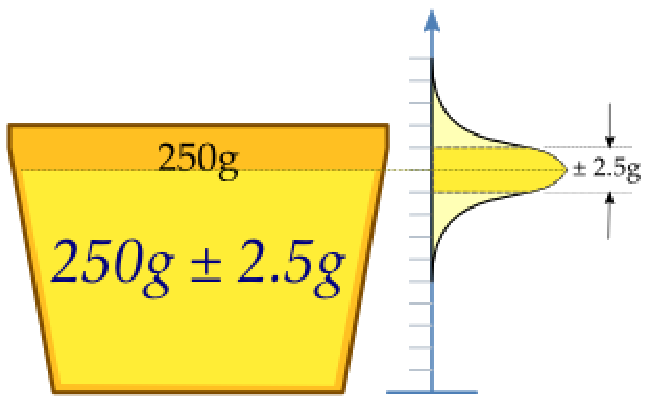
\includegraphics[scale=0.5]{ci.pdf}

\end{center}




}

\frame{
  \frametitle{Chebyshev's inequality}
 \begin{itemize}
  \item $$
    P(|X - \mu| \geq k\sigma) \leq \frac{1}{k^2}
    $$
\item The probability that a random variable lies beyond $k$
    standard deviations from its mean is less than $1/k^2$
    \begin{eqnarray*}
      2\sigma & \rightarrow & 25\% \\
      3\sigma & \rightarrow & 11\% \\
      4\sigma & \rightarrow &  6\% 
    \end{eqnarray*}
\item This is not a bound, actual probability might be (much) smaller.
 \end{itemize}


}

\frame{
  \frametitle{Chebyshev's inequality -- example}
  \begin{itemize}
  \item IQs are as a normal distribution with a $\mu$ of $100$ and a  $\sigma$ $15$
  \item What is the probability of a randomly drawn person having an IQ higher than
    $160$ or below $40$?
  \item Thus we want to know the probability of a person being more
    than $4$ standard deviations from the mean
  \item Chebyshev's inequality suggests that this will be no larger than 6\%
  \item The probability of a random draw from a bell curve being $4$
    standard deviations from the mean is on the order of $10^{-5}$ (one
    thousandth of one percent)
  \end{itemize}
}

\frame{
  \frametitle{}
  \begin{itemize}
  \item Physists say, that they are ``Six Sigma'' sure that they've discovered Higg's boson
  \item Chebyshev's inequality states that the probability of a ``Six Sigma'' event(they have not observed most ``popular'' boson) is less than $1/6^2 \approx 3\%$
  \item If normal distribution for errors is assumed, the probability of a ``six sigma'' event is on the order of $10^{-9}$ (one ten millionth of a percent)
  \end{itemize}
}
\frame{
  \frametitle{Confidence intervals}
  \begin{itemize}
   \item Sample is from normal distribution
\item We need CI for mean value
\item Variance is not unknown
  \end{itemize}
Example: we need to calculate CI for IQ level, hemoglobin, etc.

}


\frame{
  \frametitle{Confidence intervals}
% Доверительный интервал для матожидания случайной величины, распределенной по нормальному закону при известной дисперсии
 $ \Phi(x) = \frac{1}{\sqrt{2\pi}}\int_0^xe^{\frac{-t^2}{2}}dt $
\begin{enumerate}
 \item  \[
 P(|\bar{x}-a|<\delta) =2\Phi(t) = \gamma
\]
\item Using CLT: \[
 \delta = \frac{t\sigma}{\sqrt{n}}= tm,  P(\bar{x}-\delta<a<\bar{x}+\delta) =2\Phi(t) = \gamma
\]
\end{enumerate}
All we need to do is to find  $t:\Phi(t) = \frac{\gamma}{2}$
}

\frame{
  \frametitle{Confidence intervals}
  \begin{itemize}
   \item Sample is from normal distribution
\item We need CI for mean value
\item Variance is \textbf{unknown}
  \end{itemize}
Student's $t$-distribution:
$$
t = \frac{\xi_0}{\sqrt{\frac{1}{n}\sum\limits_{i=1}^n \xi_i^2}}
$$
}
\begin{frame}\frametitle{Confidence intervals for the mean}
\begin{itemize}
\item Notice that the $t$ statistic is a pivot, therefore we use it
  to create a confidence interval for $\mu$
\item Let $t_{df,\alpha}$ be the $\alpha^{th}$ quantile of the t distribution with
  $df$ degrees of freedom
  \begin{eqnarray*}
&   & 1 - \alpha \\
& = & P\left(-t_{n-1,1-\alpha/2} \leq \frac{\bar X - \mu}{S/\sqrt{n}} \leq t_{n-1,1-\alpha/2}\right) \\ \\
& = & P\left(\bar X - t_{n-1,1-\alpha/2} S / \sqrt{n} \leq \mu  
      \leq \bar X + t_{n-1,1-\alpha/2}S /\sqrt{n}\right)
  \end{eqnarray*}
\item Interval is $\bar X \pm t_{n-1,1-\alpha/2} S/\sqrt{n}$
\end{itemize}
\end{frame}
% \frame{
%   \frametitle{Confidence intervals}
% 
% }
% \frame{
%   \frametitle{Confidence intervals}
% 
% }
% % % % % % % % % % % % % % 
%  Перерыв
% % % % % % % % % % % % % % 
\frame{
\frametitle{Break}
\Huge Let's have a \textbf{break}!


}


\frame{
  \frametitle{Evidence-based medicine}
\begin{defin}
 The use of mathematical estimates of the risk of benefit and harm, derived from high-quality research on population samples, to inform clinical decision-making in the diagnosis, investigation or management of individual patients
\end{defin}

Why do we need it?
\begin{center}
\begin{tabular}{l|l}
Ancient world & Modern days\\ \hline
facies Hippocratica & obesitas \\ \hline
Plague & Heart disease

\end{tabular}
\end{center}


}

\frame{
  \frametitle{Quality of evidence}
  \begin{itemize}
\item[Level I] Evidence obtained from at least one properly designed randomized controlled trial.
\item[Level II-1] Evidence obtained from well-designed controlled trials without randomization.
\item[Level II-2] Evidence obtained from well-designed cohort or case-control analytic studies, preferably from more than one center or research group.
\item[Level II-3] Evidence obtained from multiple time series with or without the intervention. Dramatic results in uncontrolled trials might also be regarded as this type of evidence.
\item[Level III] Opinions of respected authorities, based on clinical experience, descriptive studies, or reports of expert committees.

  \end{itemize}
}

\frame{
  \frametitle{Statistical hypothesis testing}
\begin{itemize}
\item A statistical hypothesis test is a method of making decisions using data
 \item A result is called \textbf{statistically significant} if it is unlikely to have occurred by chance alone, according to a pre-determined threshold probability, the \textbf{significance level}.
\item A result that was found to be statistically significant is also called a \textbf{positive result}; conversely, a result whose probability under the null hypothesis exceeds the significance level is called a negative result or a null result.
\end{itemize}
}

\frame{
  \frametitle{Type I error and Type II error}
\begin{center}
    \begin{tabular}{ | p{3cm}  | p{3cm}  | p{3cm}  |}
    \hline
     & Null Hypothesis ($H_{0}$) is true & Alternative Hypothesis ($H_{1}$) is true  \\ \hline
     Fail to Reject Null Hypothesis & Right decision & Type II Error  \\ \hline
     Reject Null Hypothesis & Type I Error &Right decision  \\ \hline
    \end{tabular}
\end{center}
}

\frame{
  \frametitle{Statistical hypothesis testing}
\begin{itemize}
\item We start with a research hypothesis of which the truth is unknown.
\item The first step is to state the relevant null and alternative hypotheses. This is important as mis-stating the hypotheses will muddy the rest of the process. 
\item The second step is to consider the statistical assumptions being made about the sample in doing the test; for example, assumptions about the statistical independence or about the form of the distributions of the observations.
\item Decide which test is appropriate, and stating the relevant test statistic.
\item Derive the distribution of the test statistic under the null hypothesis from the assumptions. 
\item Compute from the observations the observed value tobs of the test statistic T.
\item Decide to either fail to reject the null hypothesis or reject it in favor of the alternative. 
\end{itemize}
}

\frame{
  \frametitle{}
% Проверка гипотезы о матожидании нормального распределения
\begin{enumerate}
 \item $X,Y \sim N(\mu, \sigma^2)$. 
% \item 
\item \[
       H_0:\operatorname{E}X \stackrel{d}{=} \operatorname{E}Y
      \]

\end{enumerate}

Our ``recipe'':
\begin{enumerate}
 \item 
\[
 Z = \frac{\bar{X} - \bar{Y}}{\sqrt{\frac{\sigma^2_X}{\nu_X}+\frac{\sigma^2_Y}{\nu_Y}}}
\]
% Тут $\nu_i=n_i -1$ -- количество степеней свободы в $i$-ой выборке.  Если размер выборки небольшой\footnote{тут небольшой значит меньше 30}, то необходимо знать дисперсии. Тут я предполагаю что выборки достаточно большие  и можно воспользоваться выборочными дисперсиями.
\item $\Phi(z) = \frac{1-\alpha}{2}$
\item If $|Z|< z$, $H_0$ is accepted. 
\end{enumerate}

}

\frame{
  \frametitle{}
\begin{enumerate}
 \item $X,Y \sim N(\mu, \sigma^2)$. 
% \item 
\item \[
       H_0:\operatorname{Var}X \stackrel{d}{=} \operatorname{Var}Y
      \]

\end{enumerate}
% Проверка гипотезы о дисперсии нормального распределения

% Nota Bene: $\operatorname{D}X \stackrel{d}{=} \operatorname{D}Y$ означает равенство дисперсий случайных величин, которые породили наши выборки(т.е. в терминах статистики мы сравниваем дисперсии генеральных совокупностей), а не выборочных дисперсий, которые можно сравнить тривиально: вычислить и сравнить.

Our ``recipe'':
\begin{enumerate}
 \item Calculate $\operatorname{Var}X$ and $\operatorname{Var}Y$
\item $FC=\frac{\max(\operatorname{Var}X, \operatorname{Var}Y )}{\min(\operatorname{Var}X, \operatorname{Var}Y)}$
\item Compare FC with Fisher distribution quantile with $\alpha/2$
% Сравниваем полученный критерий с квантилем обратного распределения Фищера для заданного уровня значимости деленного на два\footnote{''На пальцах:'' у нас возможны 2 способа реализации альтернативной гипотезы: одна дисперсия больше или меньше другой} и степеней свободы наших выборок. Гипотеза принимается, если квантиль больше критического значения.
\end{enumerate}
}

\frame{
  \frametitle{Example}
\begin{center}
\begin{tabular}{l|l}
Control & Experiment\\ \hline
0,027 & 0,075\\
0,036 & 0,4\\
0,1 & 0,08\\
0,12 & 0,105\\
0,32 & 0,075\\
0,45 & 0,12\\
0,049 & 0,06\\
0,105 & 0,075
\end{tabular}
\end{center}
FC: $\frac{0,0232}{0,0128}=1,8114$


Critical value for $2\alpha=0.05$ и $\nu_1=\nu_2=7$ is 4,994


}
\frame{
  \frametitle{$\chi^2$}
  \begin{itemize}
  \item Suppose that $S^2$ is the sample variance from a collection of iid
    $N(\mu,\sigma^2)$ data; then 
    $$
    \frac{(n - 1) S^2}{\sigma^2} \sim \chi^2_{n-1}
    $$
    a Chi-squared distribution with $n-1$ degrees of freedom
  \item The Chi-squared distribution is skewed and has support on $0$ to $\infty$
  \item The mean of the Chi-squared is its degrees of freedom 
  \item The variance of the Chi-squared distribution is twice the degrees of freedom
  \end{itemize}
\[
 \sum_{k=1}^N \frac{(\nu_k -n p_k)^2}{n p_i} \stackrel{d}{\rightarrow} \Xi^2_n 
\]

}

\frame{
  \frametitle{Pearson's $\chi^2$ test}
$n$ -- sample size. 

Алгоритм:
\begin{enumerate}
\item We divide the entire range of values into small intervals $\{\Delta_k\}, k = 1, \dots N$
 \item 
\[
 \chi^2_0 = \sum_{i=1}^N \frac{(v_i - np_i)^2}{np_i}
\]
 $v_k=\sum_{j=1}^nI_{\{x_j \in \Delta_k\}}$ -- frequency in $\Delta_k$. $p_k=p\{x \in \Delta_k\}$ -- probability of ``getting into'' $\Delta_k$  
 \item  $\nu = n - l -1$.l --number of parameters 
\item If $\chi^2_0<\chi^2$, then $H_0$ is accepted.
\end{enumerate}
}

\frame{
  \frametitle{Confidence interval for the variance}
Note that if $\chi^2_{n-1, \alpha}$ is the $\alpha$ quantile of the
Chi-squared distribution then
\begin{eqnarray*}
  1 - \alpha & = & P \left( \chi^2_{n-1, \alpha/2} \leq  \frac{(n - 1) S^2}{\sigma^2} \leq  \chi^2_{n-1,1 - \alpha/2} \right) \\ \\
& = &  P\left(\frac{(n-1)S^2}{\chi^2_{n-1,1-\alpha/2}} \leq \sigma^2 \leq 
\frac{(n-1)S^2}{\chi^2_{n-1,\alpha/2}} \right) \\
\end{eqnarray*}
So that 
$$
\left[\frac{(n-1)S^2}{\chi^2_{n-1,1-\alpha/2}}, \frac{(n-1)S^2}{\chi^2_{n-1,\alpha/2}}\right]
$$ \ \\ \ \\
is a $(1-\alpha)$ confidence interval for $\sigma^2$
}



% \frame{
%   \frametitle{}
% 
% }
% 
% \frame{
%   \frametitle{}
% 
% }
% 
% \frame{
%   \frametitle{}
% 
% }


\frame{
\frametitle{Dixi}

\begin{center}
\Huge Dixi\end{center}
}
\end{document}
